\subsection{Problemas}
--------------------------------------------------------
\\

\np

\begin{enumerate}[label=\alph*)]
    \item Demuestre que la fuerza neta sobre un dipolo $\Vec{p}$ en el seno de un campo eléctrico uniforme es nula. Luego, demuestre que si el campo es no uniforme, la fuerza que experimenta el dipolo se puede escribir como
    % Que es J? La expresión es equivalente a la del enunciado original?
    \[\Vec{F} = (\mathrm{J}\Vec{E})\Vec{p}\]
    donde $\mathrm{J}\Vec{E}$ es el jacobiano de $\Vec{E}$.
    \item Cuando un dipolo es sometido a la acción de un campo eléctrico uniforme, este tiende a girarlo, de modo que se orienta en la dirección del campo. Demuestre que el torque que experimenta el dipolo respecto de su centro es
    \[\Vec{\tau} = \Vec{p}\times \Vec{E}\]
    \item Demuestre que la energía potencial eléctrica de un dipolo $\Vec{p}$ en un campo eléctrico $\Vec{E}$ es
    \[U=-\Vec{p}\cdot\Vec{E}\]
\end{enumerate}

\np
 Considere un anillo circular de radio $a$, el cual almacena una carga $Q$ distribuida uniformemente. En el centro del anillo se encuentra un dipolo puntual $\Vec{p}$, alineado según el eje de la espira.
 
\begin{enumerate}[label=\alph*)]
    \item Encuentre el valor del campo eléctrico producto del dipolo en cada punto del anillo.
    \item Usando lo anterior, determine la fuerza que el dipolo ejerce sobre el anillo.
    \item Si se sabe que el campo eléctrico de un anillo en su eje está dado por:
    \[\Vec{E}_a = \frac{1}{4\pi\epsilon_o}
    \frac{Qz}{(a^2+z^2)^{3/2}}\hat{z}\]
    Calcule la fuerza que el anillo produce sobre el dipolo. Concluya hacia donde es empujado el dipolo producto del campo del anillo. ¿Cumple con la tercera Ley de Newton?
\end{enumerate}

\bigbreak

\np

Se tiene una esfera de radio $R$ con densidad de carga en su superficie no uniforme dada por $\sigma = \sigma_o(1 + \cos{\theta})$, donde $\theta$ es el ángulo polar medido con respecto al eje $z$.

\begin{enumerate}[label=\alph*)]
    \item Calcule la carga total y el momento dipolar de esta distribución. Debe determinar el valor y la orientación de dicho dipolo.
    \item Determine el potencial y el campo eléctrico producto de esta distribución de carga para puntos alejados.
    \item Encuentre explícitamente el potencial y el campo eléctrico en los puntos del eje $z$. ¿Es consistente con el resultado anterior? Discuta su resultado.
\end{enumerate}
\bigbreak

\np

Una corteza cilíndrica de radio interior $a$ y exterior $b$ está hecha de un material dieléctrico polarizado según la ley $\Vec{P} = k\rho\hat{\rho}$. No hay más cargas en el sistema.

\begin{enumerate}[label=\alph*)]
    \item Calcule las densidades de carga de polarización en el sistema. ¿Cuánto vale la carga total de polarización?
    \item Determine los campos $\Vec{D}$ y $\Vec{E}$ en todo el espacio.
    \item Determine el valor del potencial eléctrico en todo el espacio.
\end{enumerate}

\bigbreak

\np

Entre dos placas metálicas planas y paralelas, de sección $S$ y separadas una distancia $a$, se encuentra un dieléctrico que presenta polarización permanente, de forma que en él $\Vec{P} = \Vec{P}_0$, siendo $\Vec{P}_0$ un vector uniforme, en la dirección perpendicular a las placas.

\begin{enumerate}[label=\alph*)]
    \item Inicialmente las placas están descargadas. Si se conectan mediante un voltímetro, ¿cuál es la diferencia de potencial entre las placas que medirá este?
    \item  Suponga que las dos placas se conectan mediante un hilo conductor, ¿cuánta carga se almacena en cada placa conductora?
    \item Calcule cómo cambian los resultados anteriores si la polarización del dieléctrico no es constante, sino que depende del campo como $\Vec{P} = \Vec{P}_0 + \epsilon_o
    \mathcal{X}_e\Vec{E}$.
\end{enumerate}

\bigbreak
\np

La polarización de todo el espacio, excepto para $r < R$, está dada por $\Vec{P} = P_0\hat{r}$, donde $P_0$ es constante y $\hat{r}$ es la dirección radial. Determine las cargas de polarización y el campo eléctrico en todo el espacio.

\bigbreak

\np% P2 C2 Mancilla 2018

Se tiene una esfera, de radio $R$, de un material
dieléctrico de susceptibilidda eléctrica $\mathcal{X}$, alrededor de la cual hay vacío. Si se aplica a la esfera un campo eléctrico uniforme $\Vec{E}_0 = E_0\hat{z}$, esta produce una polarización inicial igual a $\Vec{P}_0 = \epsilon_o\mathcal{X}\Vec{E}_0$.

\begin{enumerate}[label=\alph*)]
    \item Determine las cargas de polarización asociadas a $\Vec{P}_0$
    \item Se sabe que una esfera polarizada uniformemente produce en su interior un campo eléctrico uniforme. A partir de las cargas de polarización, calcule el campo eléctrico que producen en el centro de la misma esfera. Luego concluya que
    \[E_1 = -\frac{1}{3\epsilon_o}\Vec{P}_0\]
    donde $\Vec{E}_1$ es el campo eléctrico en el interior de la esfera generado por la polarización inicial $\Vec{P}_0$
    \item De esta forma, la materia no está sometida sólo al campo $\Vec{E}_0$, sino a la suma de $\Vec{E}_0$ y $\Vec{E}_1$. A la polarización habrá que sumar, por tanto, una corrección $\Vec{P}_1$ generada por $\Vec{E}_1$. Determine $\Vec{P}_1$.
    \item El proceso sigue entonces añadiendo más y más términos, hasta tener una serie infinita de ellos. El campo eléctrico total será la suma de esta serie. Determine la serie en cuestión y utilizando la serie geométrica $\frac{1}{1+x} = 1 - x + x^2 - x^3 + \cdots$ demuestre que el campo eléctrico al interior de la esfera es
    \[\Vec{E}=\frac{1}{1+\frac{\mathcal{X}}{3}}\Vec{E}_0\]
\end{enumerate}


\np

Muchos materiales dieléctricos presentan lo que se conoce como saturación, lo que quiere decir que la polarización alcanza un máximo. En un material de este tipo el comportamiento se puede aproximar mediante la gráfica de la figura. La polarización crece linealmente con el campo eléctrico hasta un valor máximo $\Vec{P_0}=\epsilon_o\mathcal{X}_e\Vec{E}_0$. Supongamos que en el centro de una esfera de radio $a$ de un material así se coloca una carga puntual $q$.

\begin{enumerate}[label=\alph*)]
    \item Determine los campos $\Vec{E}$ , $\Vec{P}$ y $\Vec{D}$ en todo el espacio.
    \item Determine las densidades de carga de polarización. ¿Y la carga total de polarización?
    \item ¿Cómo cambiarían sus respuestas si el dieléctrico no se saturase, esto es, si $\Vec{P_0}=\epsilon_o\mathcal{X}_e\Vec{E}_0$ siempre?
\end{enumerate}

\begin{figure}[H]
    \centering
    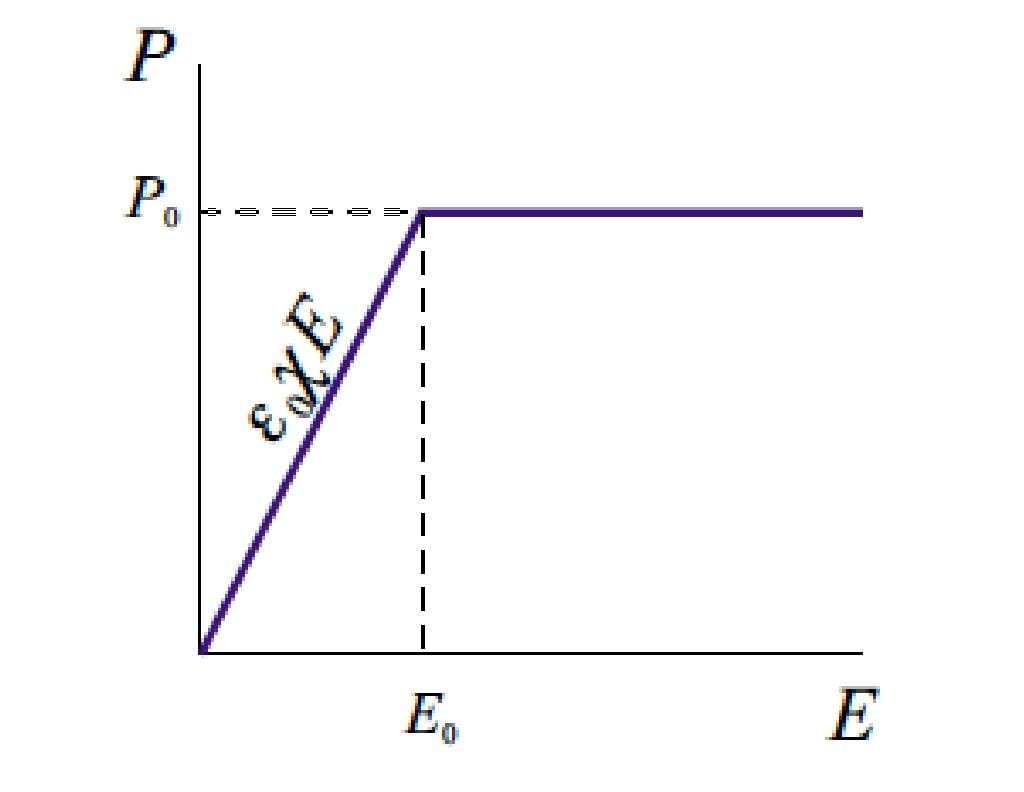
\includegraphics[width=0.54\textwidth]{Electroestática/Dipolos/grafico.jpeg}
\end{figure}

\bigbreak
\np % C2 Mancilla 2017-1 P1

Se tiene una esfera conductora de radio $R$, la cual se encuentra aislada y almacena una carga neta $Q$.

\begin{enumerate}[label=\alph*)]
    \item Si la esfera se encuentra en el vacío. Indique la energía almacenada en el sistema. % P.6.5
    \item  Suponga que, sin descargar la esfera, esta se recubre con una capa de espesor $a$ de un material dieléctrico lineal de permitividad $\epsilon$. Determine la nueva energía almacenada en el sistema. ¿Cómo se explica el cambio en la energía?
    \item  Determine la polarización del material dieléctrico y las densidades de cargas de polarización.
    \item Si en lugar de una esfera aislada, tenemos una esfera conectada a un generador que fija su potencial en un valor $V_0$, ¿cuál es la energía antes y después del recubrimiento? ¿Cómo se interpreta el cambio de energía en este caso?
\end{enumerate}

Considere que para un dieléctrico lineal, la energía electrostática almacenada en el sistema es

\[U = \frac{1}{2}\int\Vec{E}\cdot\Vec{D}\,dV\]

\bigbreak

\np

Se tienen dos placas conductoras de superficie $\mathcal{S}$ situadas paralelamente y separadas una distancia $a$. Entre ellas se coloca un dieléctrico lineal con una permitividad variable de la forma

\[\epsilon(z) = \epsilon_1 + (\epsilon_2-\epsilon_1)\frac{z}{a}\]

donde $z$ es la coordenada perpendicular a las placas, con $z=0$ en la placa inferior. Este material es denominado un medio estratificado. Despreciando los efectos de borde, determine:

\begin{enumerate}[label=\alph*)]
    \item Los campos $\Vec{E}$ , $\Vec{P}$ y $\Vec{D}$ en todos los puntos entre las placas cuando entre estas se establece una diferencia de potencial $V_0$.
    \item Las densidades de carga de polarización (tanto superficial como volumétrica).
    \item Determine la energía almacenada en el sistema.
\end{enumerate}
\bigbreak
\np

Dos condensadores cilíndricos de radio interior $a$ y exterior $c$, y largo $L$, han sido llenados con dos materiales dieléctricos de permitividades $\epsilon_1$ y $\epsilon_2$ de distinta forma, como se muestra en la figura.

\begin{figure}[H]
    \centering
    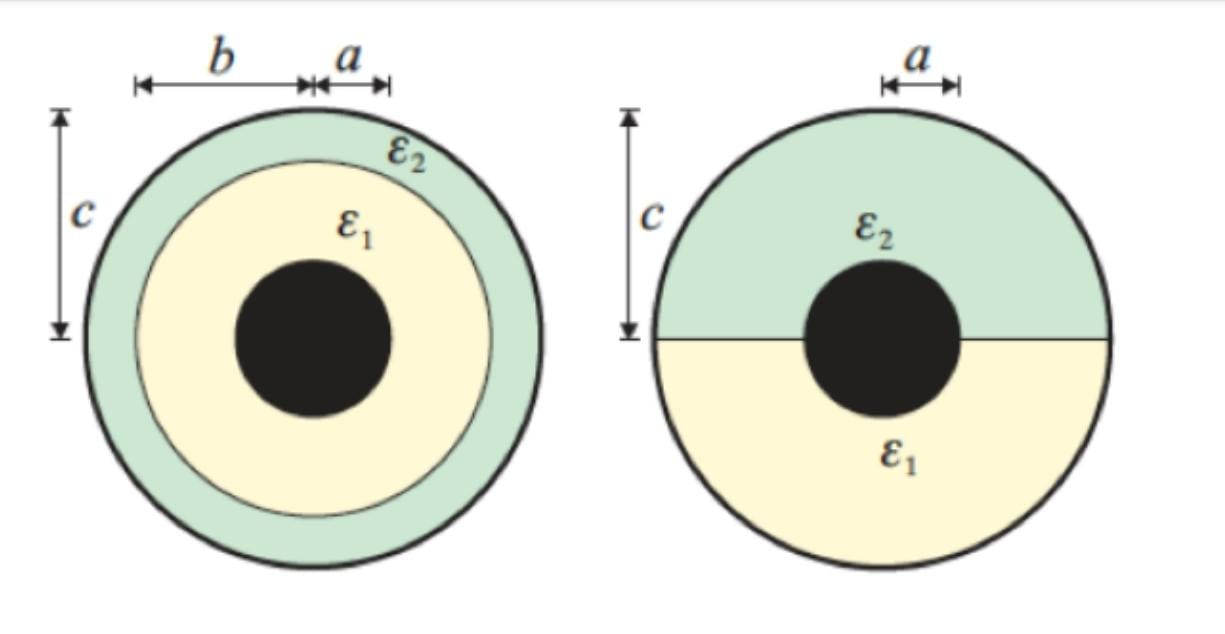
\includegraphics[width=0.7\textwidth]{Electroestática/Dipolos/Cilindros.jpeg}
\end{figure}

\begin{enumerate}[label=\alph*)]
    \item Determine los campos $\Vec{E}$ , $\Vec{P}$ y $\Vec{D}$ entre las placas, para cada configuración.
    \item Calcule la capacitancia de los dos sistemas, para cada configuración.
\end{enumerate}
\bigbreak

\np
Una esfera conductora de radio $a$ se encuentra conectada a una fuente de poder de valor $V_0$. La esfera se encuentra semi-sumergida en un líquido dieléctrico lineal de permitividad $\epsilon$.

\begin{enumerate}[label=\alph*)]
    \item Determine los campos $\Vec{E}$ , $\Vec{P}$ y $\Vec{D}$ en todo el espacio.
    \item Determine las distribuciones de carga libre y de polarización que hay en el sistema descrito.
    \item Calcule la energía electrostática almacenada en el sistema.
    \item Si, sin desconectar la fuente, se retira el líquido dieléctrico, ¿cuánto cambia la energía almacenada? ¿Cuánto trabajo realiza la fuente de poder?
\end{enumerate}

\begin{figure}[H]
    \centering
    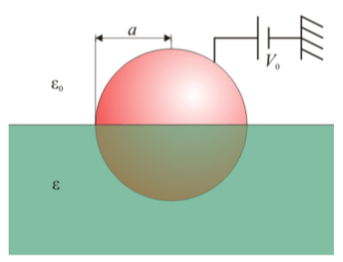
\includegraphics[width=0.4\textwidth]{Electroestática/Dipolos/EsferaP_8_12.png}
\end{figure}

\newpage